% Overview of assurance argument structure
The high-level structure of our CASE assurance pattern is inspired by the D-MILS argument pattern~\cite{dmils}, in which system dependability properties are assured via modules arguing component, compositional, and implementation correctness.  
Although verifying functional, safety, and other dependability properties is necessary for a comprehensive system assurance case, the CASE pattern presented here only addresses cyber-resiliency.  The intention is for the resulting assurance argument to be integrated into a full system dependability assurance case, when necessary.

The high-level CASE argument structure is depicted in Fig.~\ref{fig:top-level}, with the top-level goal being ``The system is acceptably cyber-resilient".  
This goal is then substantiated by arguments that cyber-resiliency requirements have been appropriately identified and then satisfied, both in the system model and the \textit{realization} of the system model as a built, deployable system.

\begin{figure}[h] 
	\centering 
	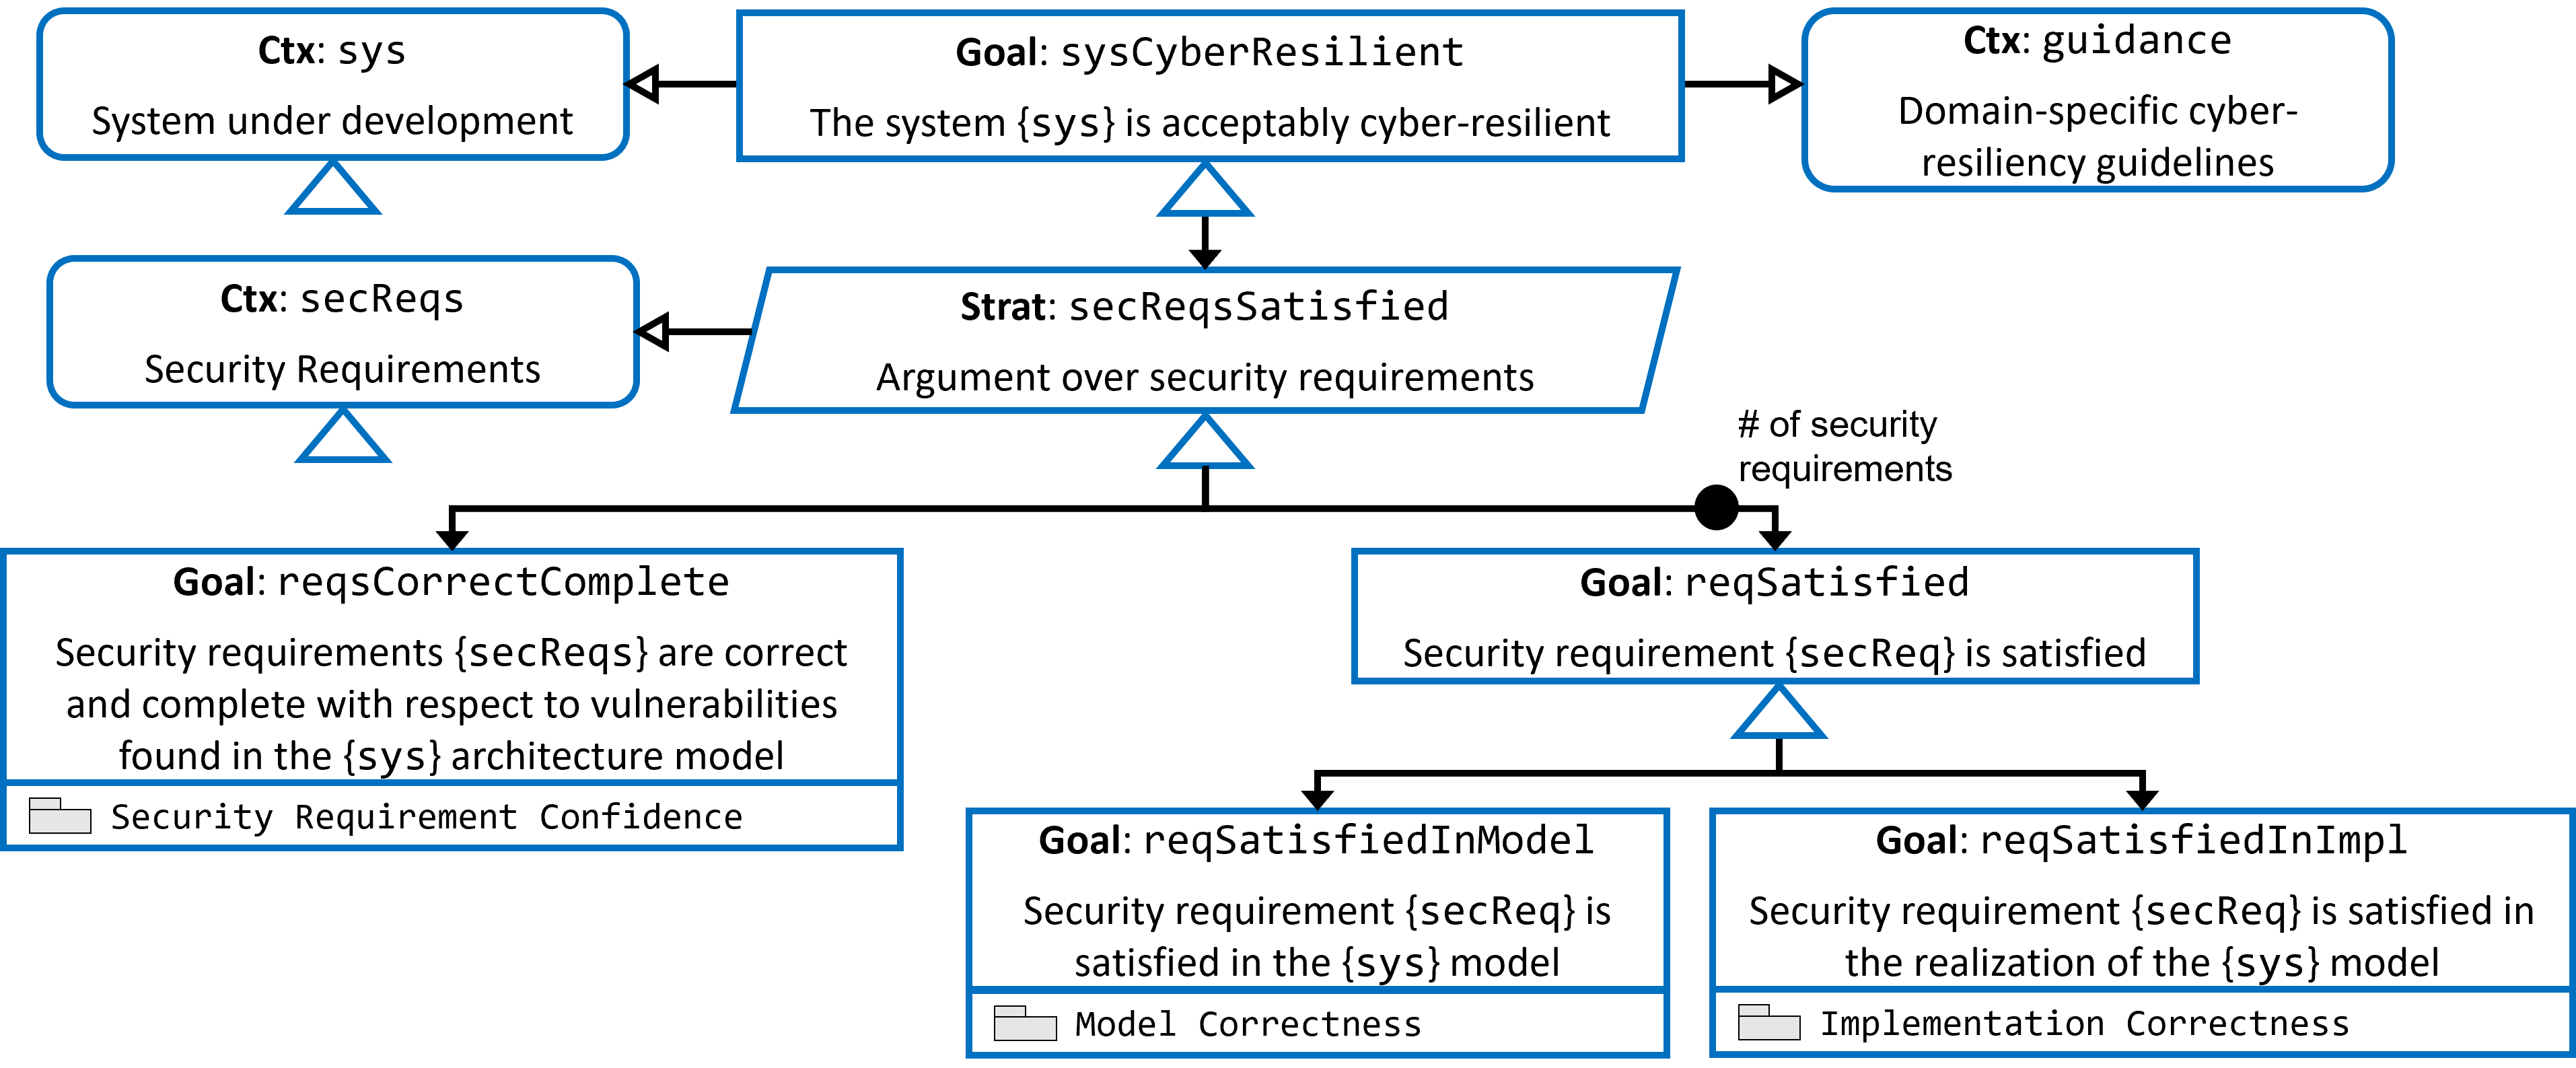
\includegraphics[width=\textwidth]{figs/top-level.png}
	\caption{Top-level assurance pattern structure.}
	\label{fig:top-level} 
\end{figure}


% Describe at a high-level how each workflow step should be assured.  Refer to figure.  Then dive into BriefCASE assurance pattern.

% Security requirements are correct and complete
\subsection{Cyber Requirement Correctness and Completeness}
%BriefCASE currently includes two cybersecurity plug-ins, GearCASE~\cite{gearcase2020} and DCRYPPS~\cite{dcrypps2019}, that analyze an AADL model and output a set of cyber requirements corresponding to vulnerabilities detected in the model.  
%BriefCASE maintains the generated requirements within the framework as assurance goals using the Resolute tool~\cite{resolute2014}.  
%In addition to providing an AADL annex grammar for representing assurance cases, Resolute includes an evaluation engine for determining whether sufficient evidence exists (both internal and external to the AADL workspace) to support assurance claims.  
%Because BriefCASE manages the development artifacts associated with the CASE workflow, it automatically provides Resolute with instructions on how those artifacts can be used to support specific cyber-resiliency goals.
%Resolute generates assurance arguments in a tree format, but also supports export to graphical tools such as AdvoCATE~\cite{advocate}.  


The assurance argument for cybersecurity requirement correctness and completeness is shown in Fig.~\ref{fig:req-correct-complete}.  
%
In the figure, it can be seen that in order to support the claim, we must provide evidence that the full set of cyber requirements passed through a review process, were imported into the BriefCASE environment as Resolute goals or omitted with rationale, and that successive analyses on updated versions of the model finds no new vulnerabilities.  The latter reflects the iterative step in the workflow (depicted by the left-pointing arrow in Fig.~\ref{fig:workflow}), in which a modified model must be re-analyzed after applying a mitigation for a previously generated requirement.  This is necessary in order to demonstrate that the mitigation of one vulnerability does not inadvertently introduce other vulnerabilities.  To argue that the current model was analyzed appropriately, we must be able to demonstrate first that the model is well-formed; that is, it complies with modeling guidelines, that the analysis was indeed performed on the current version of the model, and that the analysis does not produce any new applicable requirements.

\begin{figure}[h] 
	\centering 
	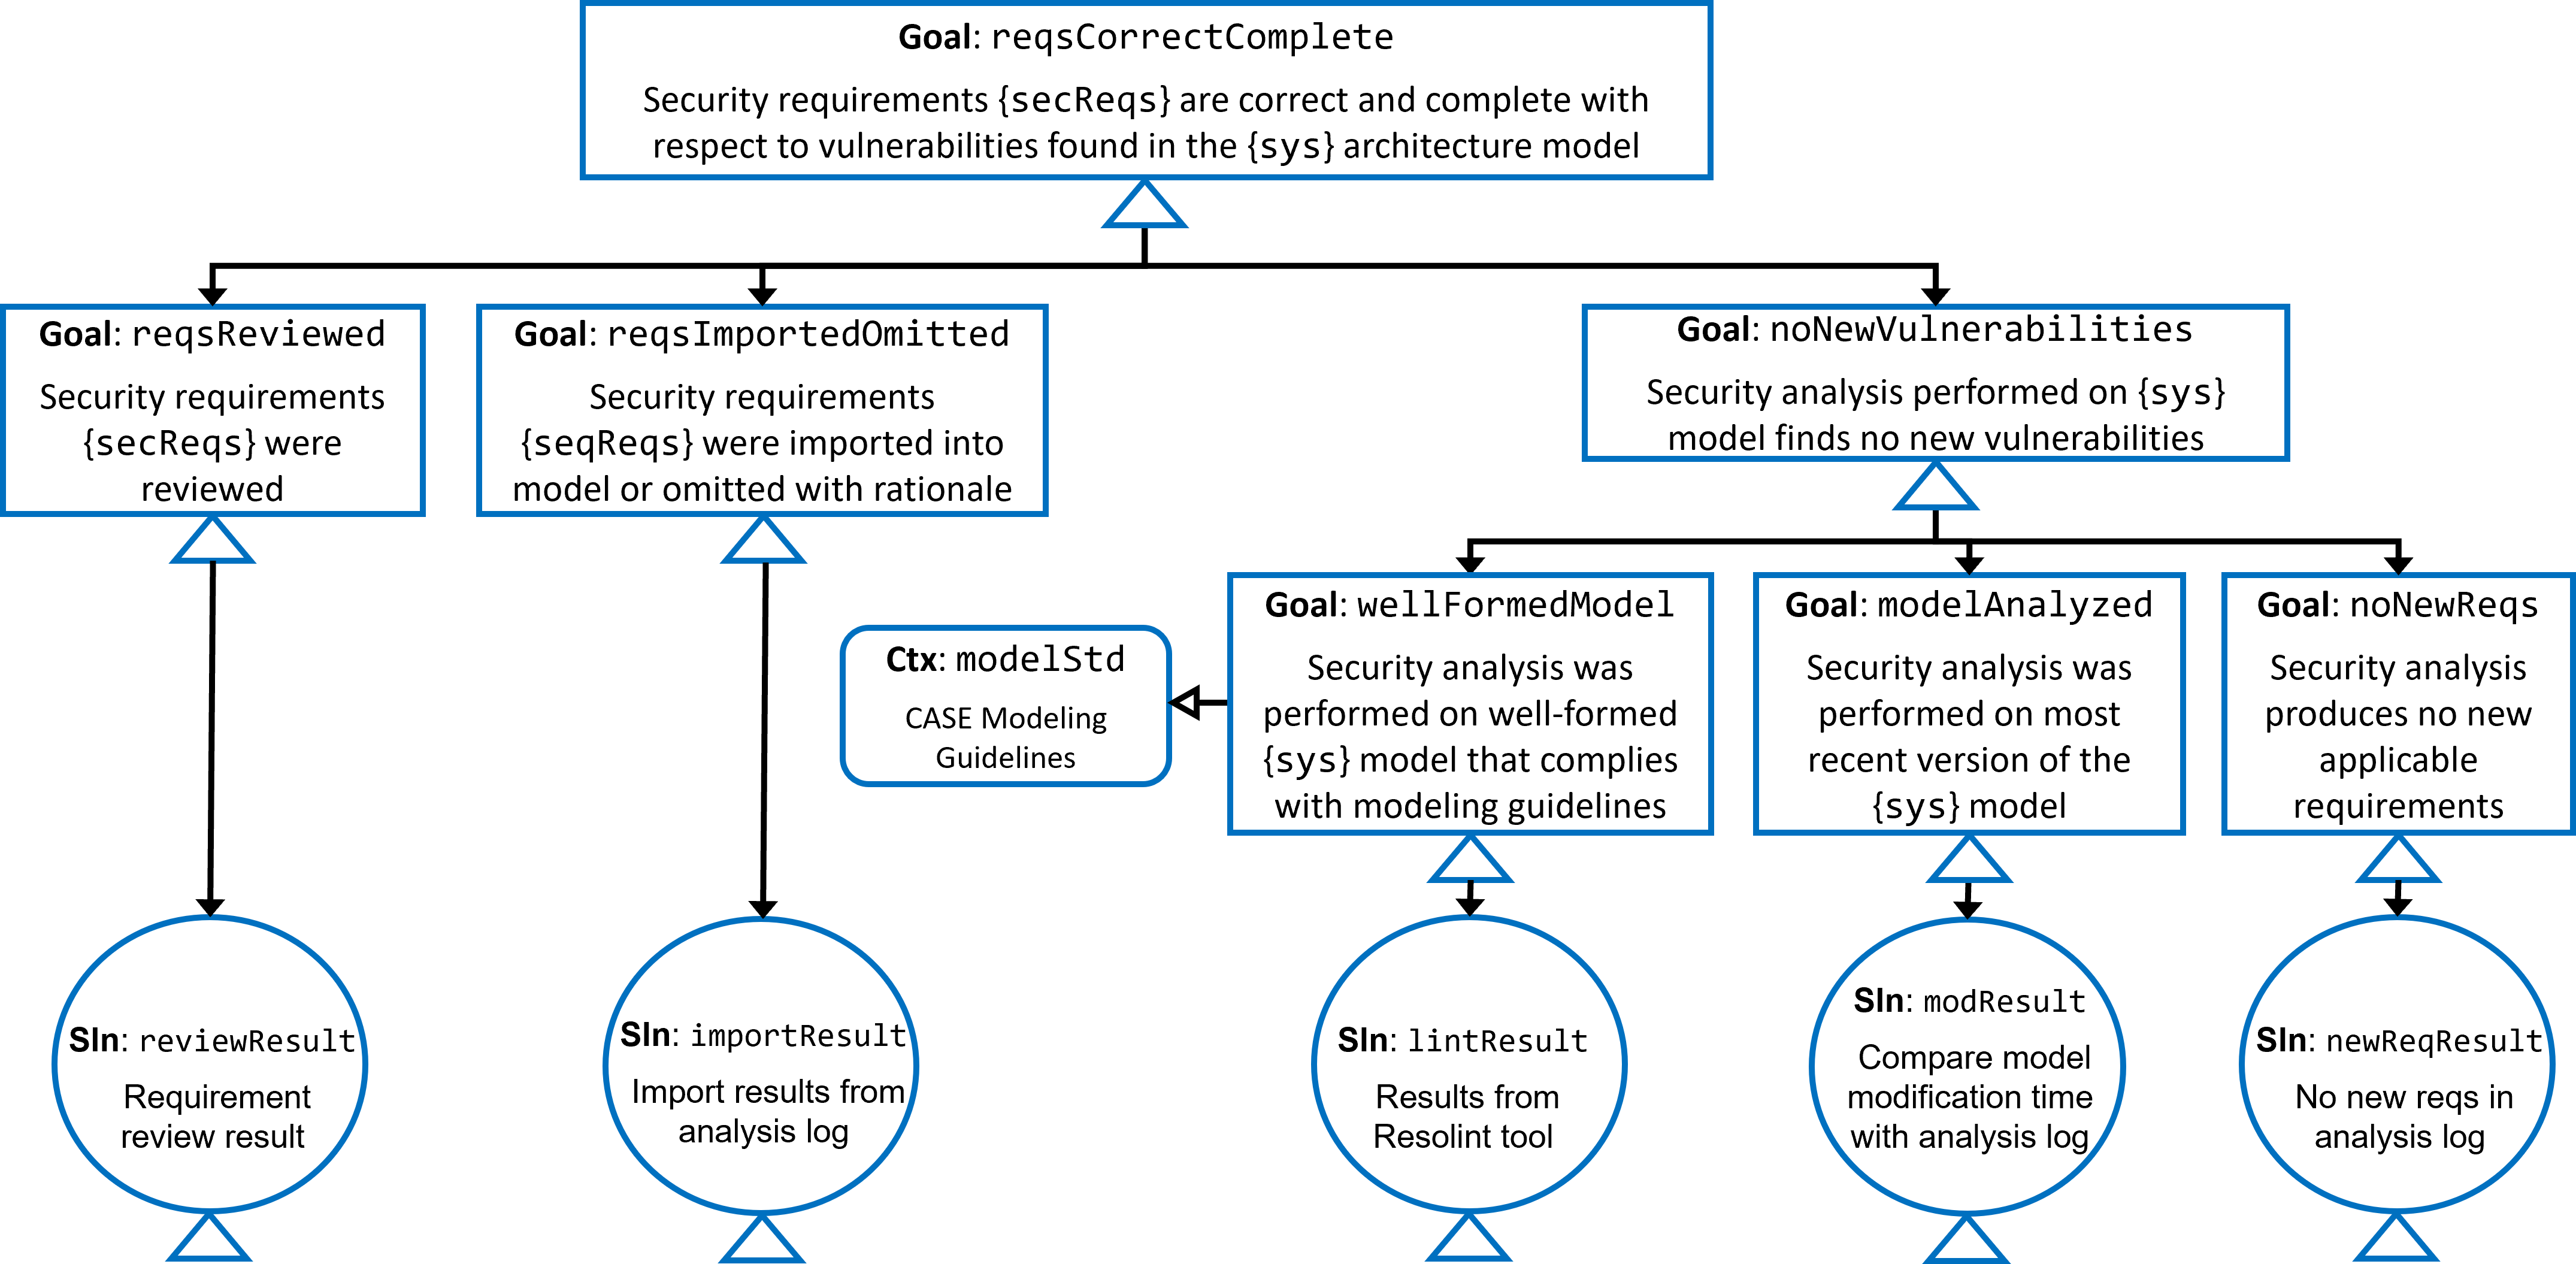
\includegraphics[width=\textwidth]{figs/req-correct-complete.png}
	\caption{Assurance pattern for security requirement correctness and completeness.}
	\label{fig:req-correct-complete} 
\end{figure}

% Model assurance
\subsection{Cyber Requirements are Satisfied in the System Model}
\label{sec:requirements-satisfied-in-model}
BriefCASE includes a library of automated model transformations corresponding to common cyber requirement classes.  Each transformation modifies the model to harden it against a specific vulnerability, thereby mitigating the associated threat and addressing the driving requirement.  In addition, the transformations automatically update the corresponding Resolute goals with instructions that enable Resolute to evaluate whether the goal is supported by the necessary evidence.

% NOT SURE HOW MUCH SPACE WE WILL HAVE HERE.
% USE FILTER AS EXAMPLE
% OTHERWISE, JUST REFERENCE DESTION PAPER 
Because the transformations modify the architecture model in different ways, assuring that a specific requirement is satisfied in the model will be argued according to a transformation-specific pattern.  For example, the well-formed message requirement (described in Section~\ref{sec:briefcase}) can be addressed by inserting a filter on the communication channel upstream of the target component.  The corresponding assurance pattern for this mitigation is shown in Fig.~\ref{fig:filter}.  Here, we argue that the well-formed message requirement has been satisfied in the model by showing that formal verification passed on the current version of the model, that a filter is appropriately inserted upstream of the target component, and that the filter cannot be bypassed.  Assurance patterns corresponding to all the BriefCASE model transformations have been defined and are packaged with the framework.  Due to space limitations we do not include them here, but instead refer the reader to the BriefCASE User's Guide~\cite{BriefCASE-user-guide}.

\begin{figure}[h] 
	\centering 
	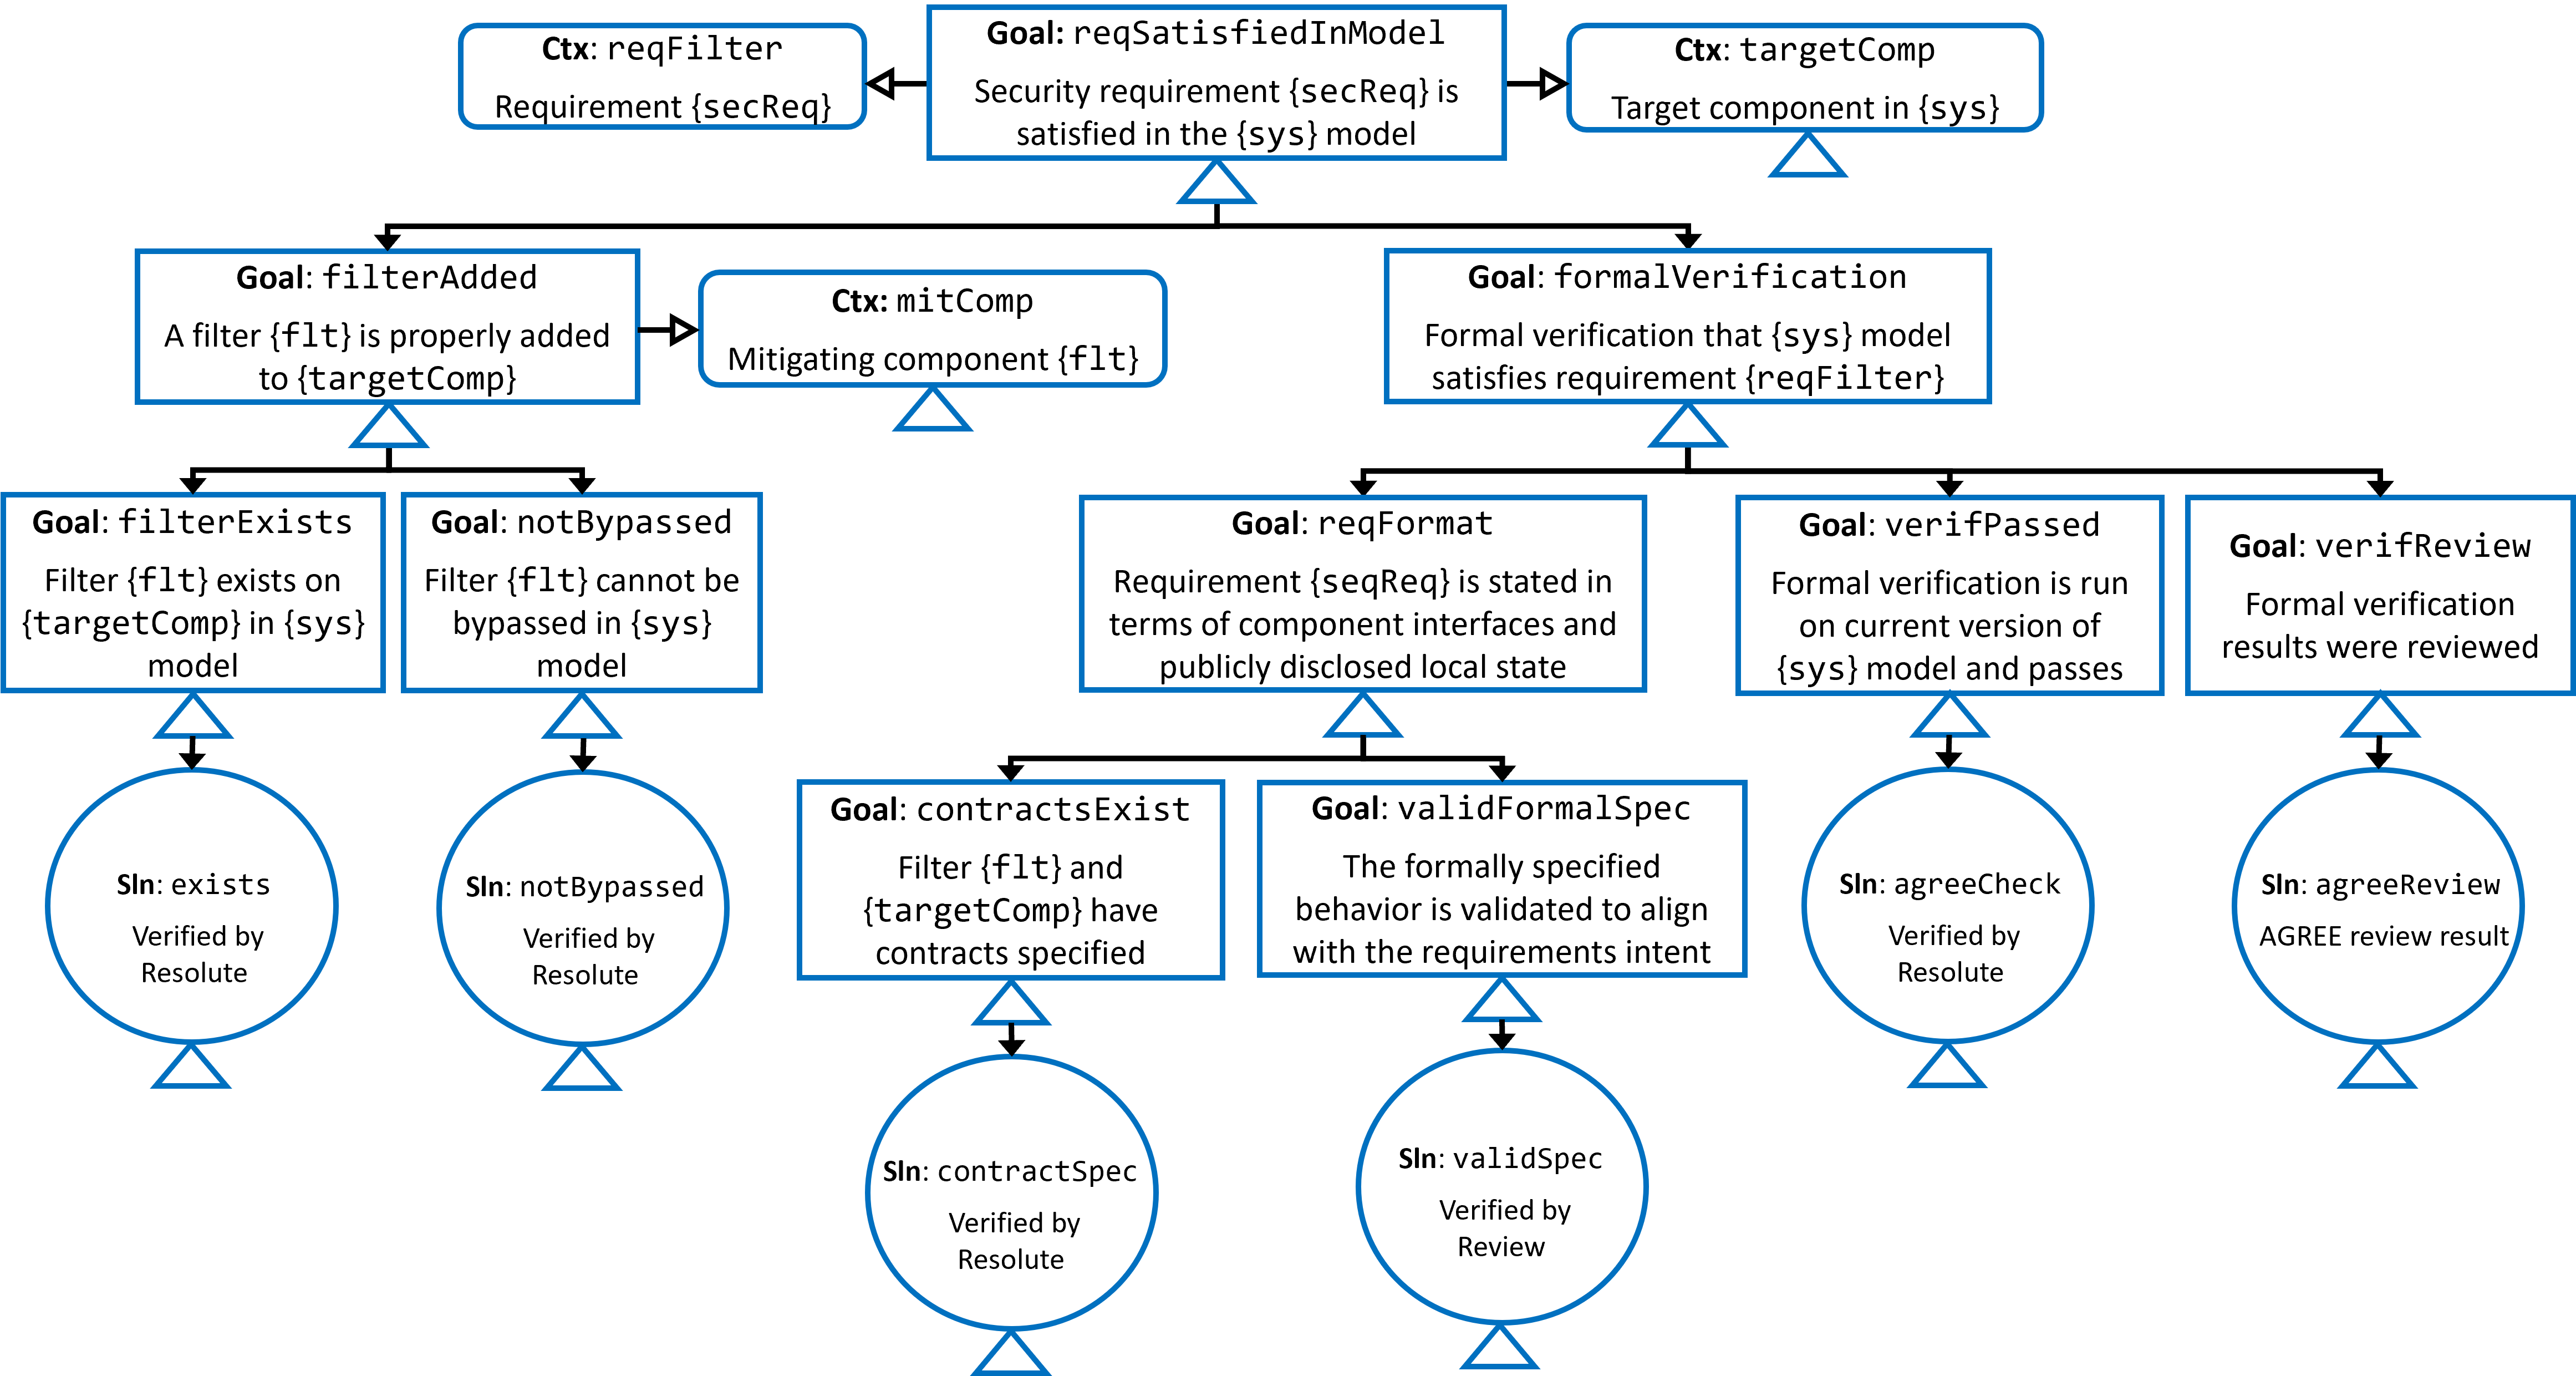
\includegraphics[width=\textwidth]{figs/filter.png}
	\caption{Pattern for assuring proper filter mitigation in the architecture model.}
	\label{fig:filter} 
\end{figure}

% Implementation assurance
\subsection{Cyber Requirements are Satisfied in the Realization of the System Model}
% Where BriefCASE implementations can come from (legacy/manual implementation, SPLAT synthesis, pre-packaged - Attestation, seL4, HAMR)

In the CASE workflow, a software component implementation could have various origins.  It could be legacy, third-party, or manually implemented code. It could also be generated from a behavioral model such as Simulink or be synthesized directly from the component's contract.  In BriefCASE, the latter is performed by the SPLAT tool, which synthesizes the implementation of high-assurance components in CakeML directly from a formal assume-guarantee contract specified in the AADL component's AGREE annex.  In addition to providing a formally verified compiler, CakeML enables SPLAT to generate a proof that the synthesized implementation is correct with respect to the component's formal contract.

Application infrastructure code and the operating system itself must also be implemented and integrated into a deployable system.  BriefCASE employs the HAMR build tool, which generates the infrastructure code, along with correspondence proofs that the inter-component connections specified in the model are maintained in the implementation and that no new connections have been created.  For high-assurance systems, this is made possible in part by building to a target platform running the formally verified seL4, which provides time and space partitioning guarantees.

To help ensure that (a) system executables conform to AADL model semantics and (b) semantics are consistent across different AADL-aligned code generation frameworks, AADL defines principles for structuring application code and specifies key semantic steps in the form of Run-Time Services (RTS). AADL RTS are library functions, some of which are called by AADL infrastructure code while others may be called by application code (e.g., to access values on component ports). The AADL RTS also provide an abstraction layer: details of the underlying platform execution may be hidden behind RTS APIs, allowing a significant portion of AADL application threading and infrastructure code to be platform independent. HAMR makes heavy use of these concepts to achieve its support for multiple platforms.

Working off of an AADL instance model as generated by OSATE, HAMR generates a CAmkES specification of the deployment topology and other kernel configuration information. For each AADL thread, HAMR generates infrastructure code that implements the AADL thread dispatch semantics. This includes (a) infrastructure code for linking entry point application code to seL4 underlying scheduling framework, for implementing the storage associated with ports, and for realizing the buffering and notification semantics associated with event and event data ports; and (b) developer-facing code including thread code skeletons in which the developer will write application code, and port APIs that the application code uses to send and receive messages over ports.

%\begin{figure}[h] 
%	\centering 
%	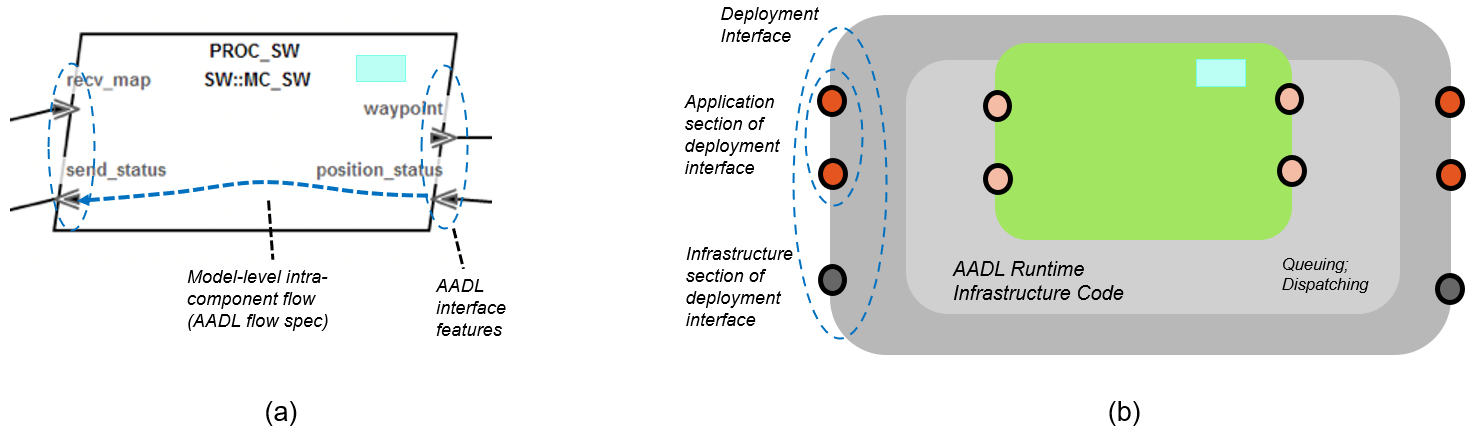
\includegraphics[width=\textwidth]{figs/deployment-interface.png}
%	\caption{(a) Example AADL component interface features and disclosed component state. (b) Schematic of deployed component, with notion of observation points.}
%	\label{fig:deployment-interface} 
%\end{figure}

The structure of the \textit{model realization} branch of the assurance pattern (partially shown in Fig.~\ref{fig:req-satisfied-in-model-realization}) therefore necessarily focuses on evidence of correctness in terms of behaviors observed at deployment observation points associated with the BriefCASE workflow. 

\begin{figure}[h] 
	\centering 
	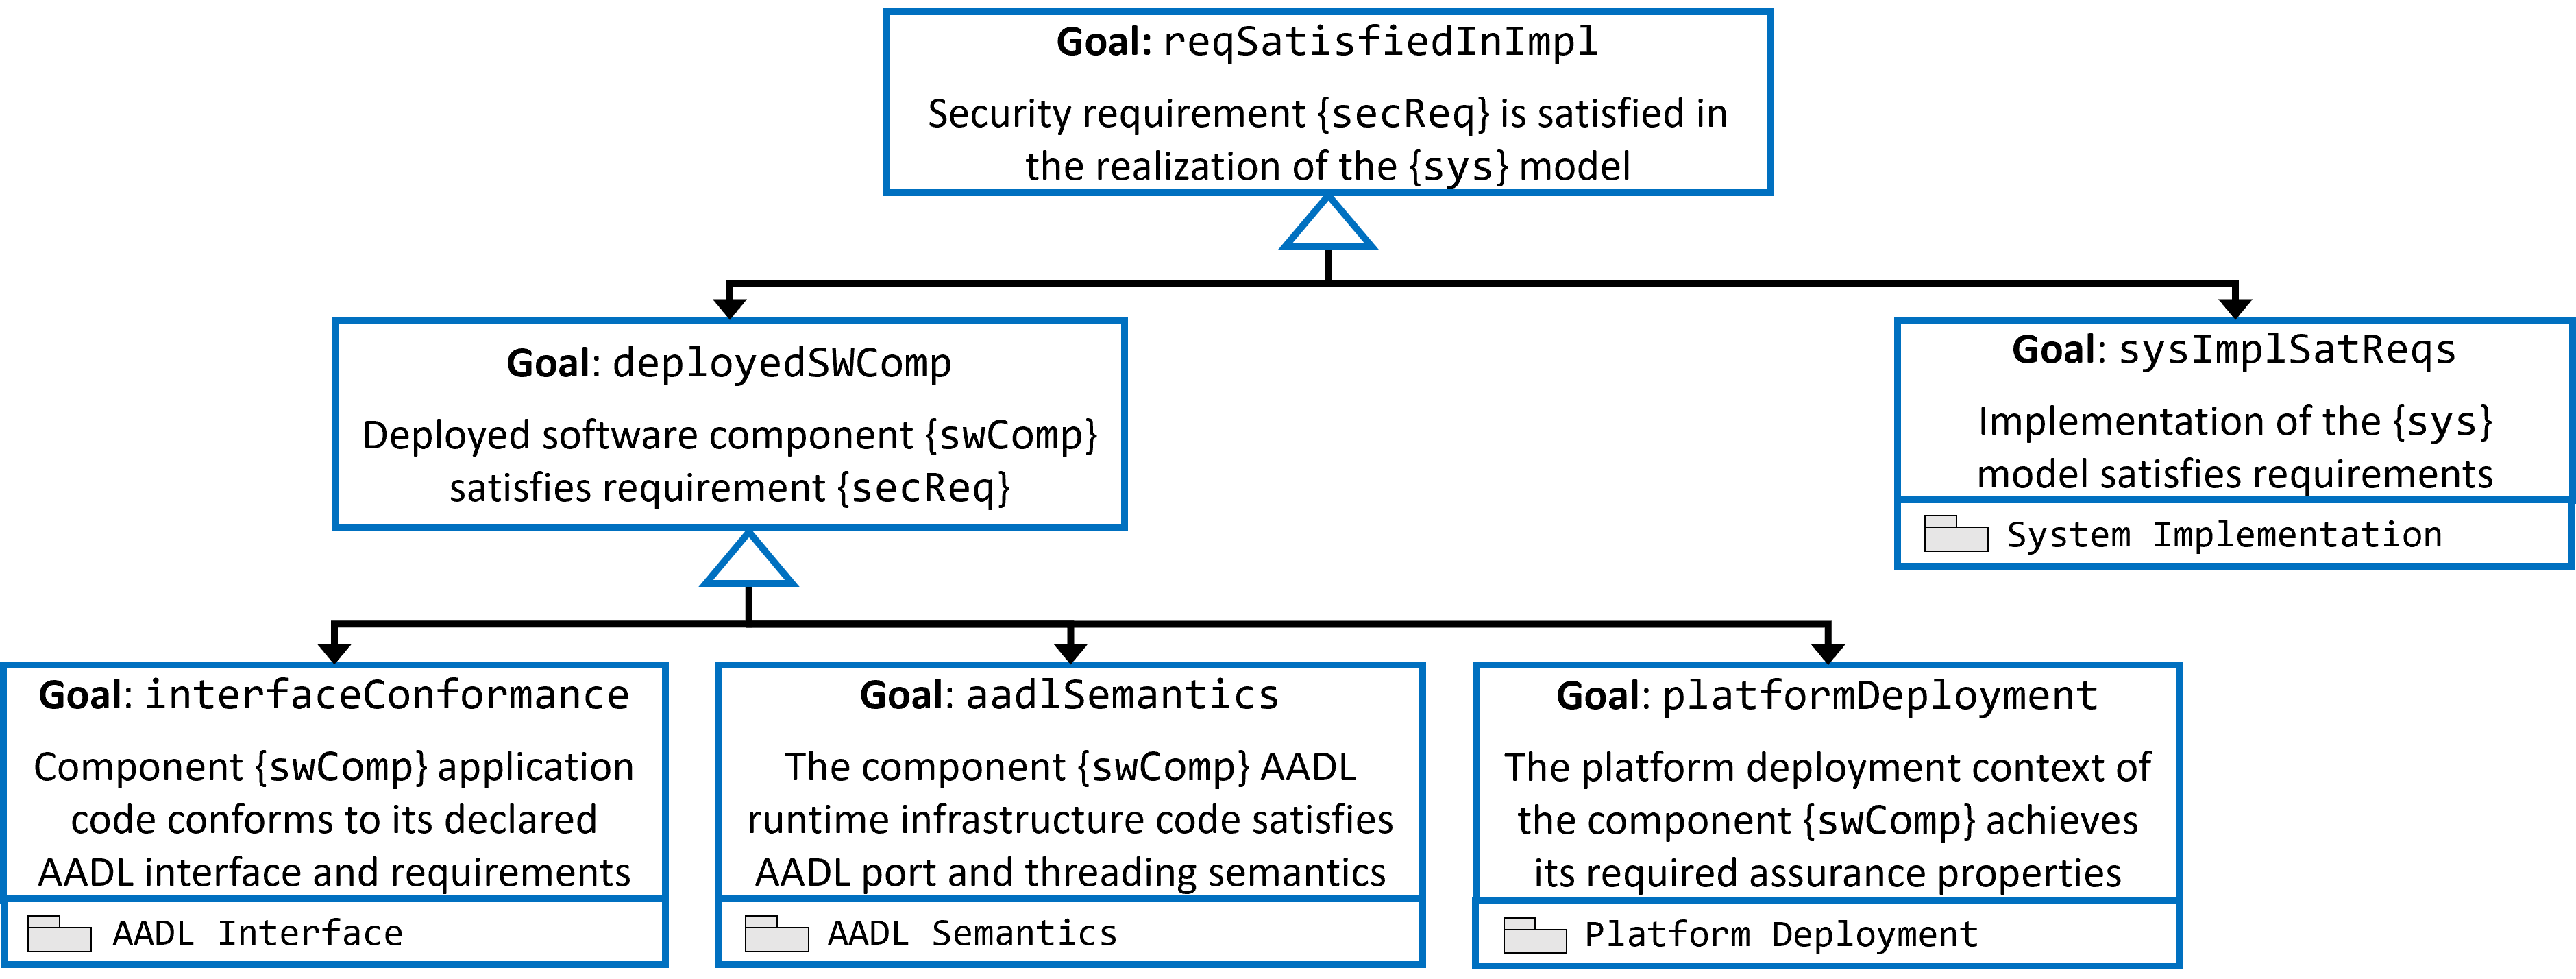
\includegraphics[width=\textwidth]{figs/req-satisfied-in-model-realization.png}
	\caption{Assurance pattern for arguing the requirement is satisfied in the realization of the model.}
	\label{fig:req-satisfied-in-model-realization} 
\end{figure}

To support the claim that the deployed software components satisfy their cyber requirements, we produce an argument for each applicable component.
%in Figure~\ref{fig:req-satisfied-in-model-realization}
We first desire evidence that the requirement is stated in terms of the component's AADL interface and publicly disclosed state. 
Although demonstrating that requirements are stated in terms of the component's interface is not strictly necessary in the general case, it is included in this pattern for confidence that the CASE workflow was followed correctly.  In the case of a formally specified functional requirement, this may be substantiated with evidence that the formally specified behavior has been validated to align with the requirement's intent (i.e., failure and success cases for the formal specification are provided that cover the concepts reflected in the requirements) and the requirement is correctly specified in the formal specification language (i.e., requirement review).

We must then demonstrate that the component application code conforms to both its declared interface and requirements (goal \texttt{G???}), that the component's AADL runtime infrastructure code satisfies AADL port and threading semantics (goal \texttt{G???}), and that the component's platform deployment context achieves its required assurance properties is needed (goal \texttt{G???}).  

%Furthermore, the component's application code must conform to its declared interface and requirements.  
Goal \texttt{G???} is substantiated by the argument in Fig.~\ref{fig:code-conforms-to-interface-and-requirements}.
\todo{Complete this argument description and required evidence}

\begin{figure}[h]
	\centering 
	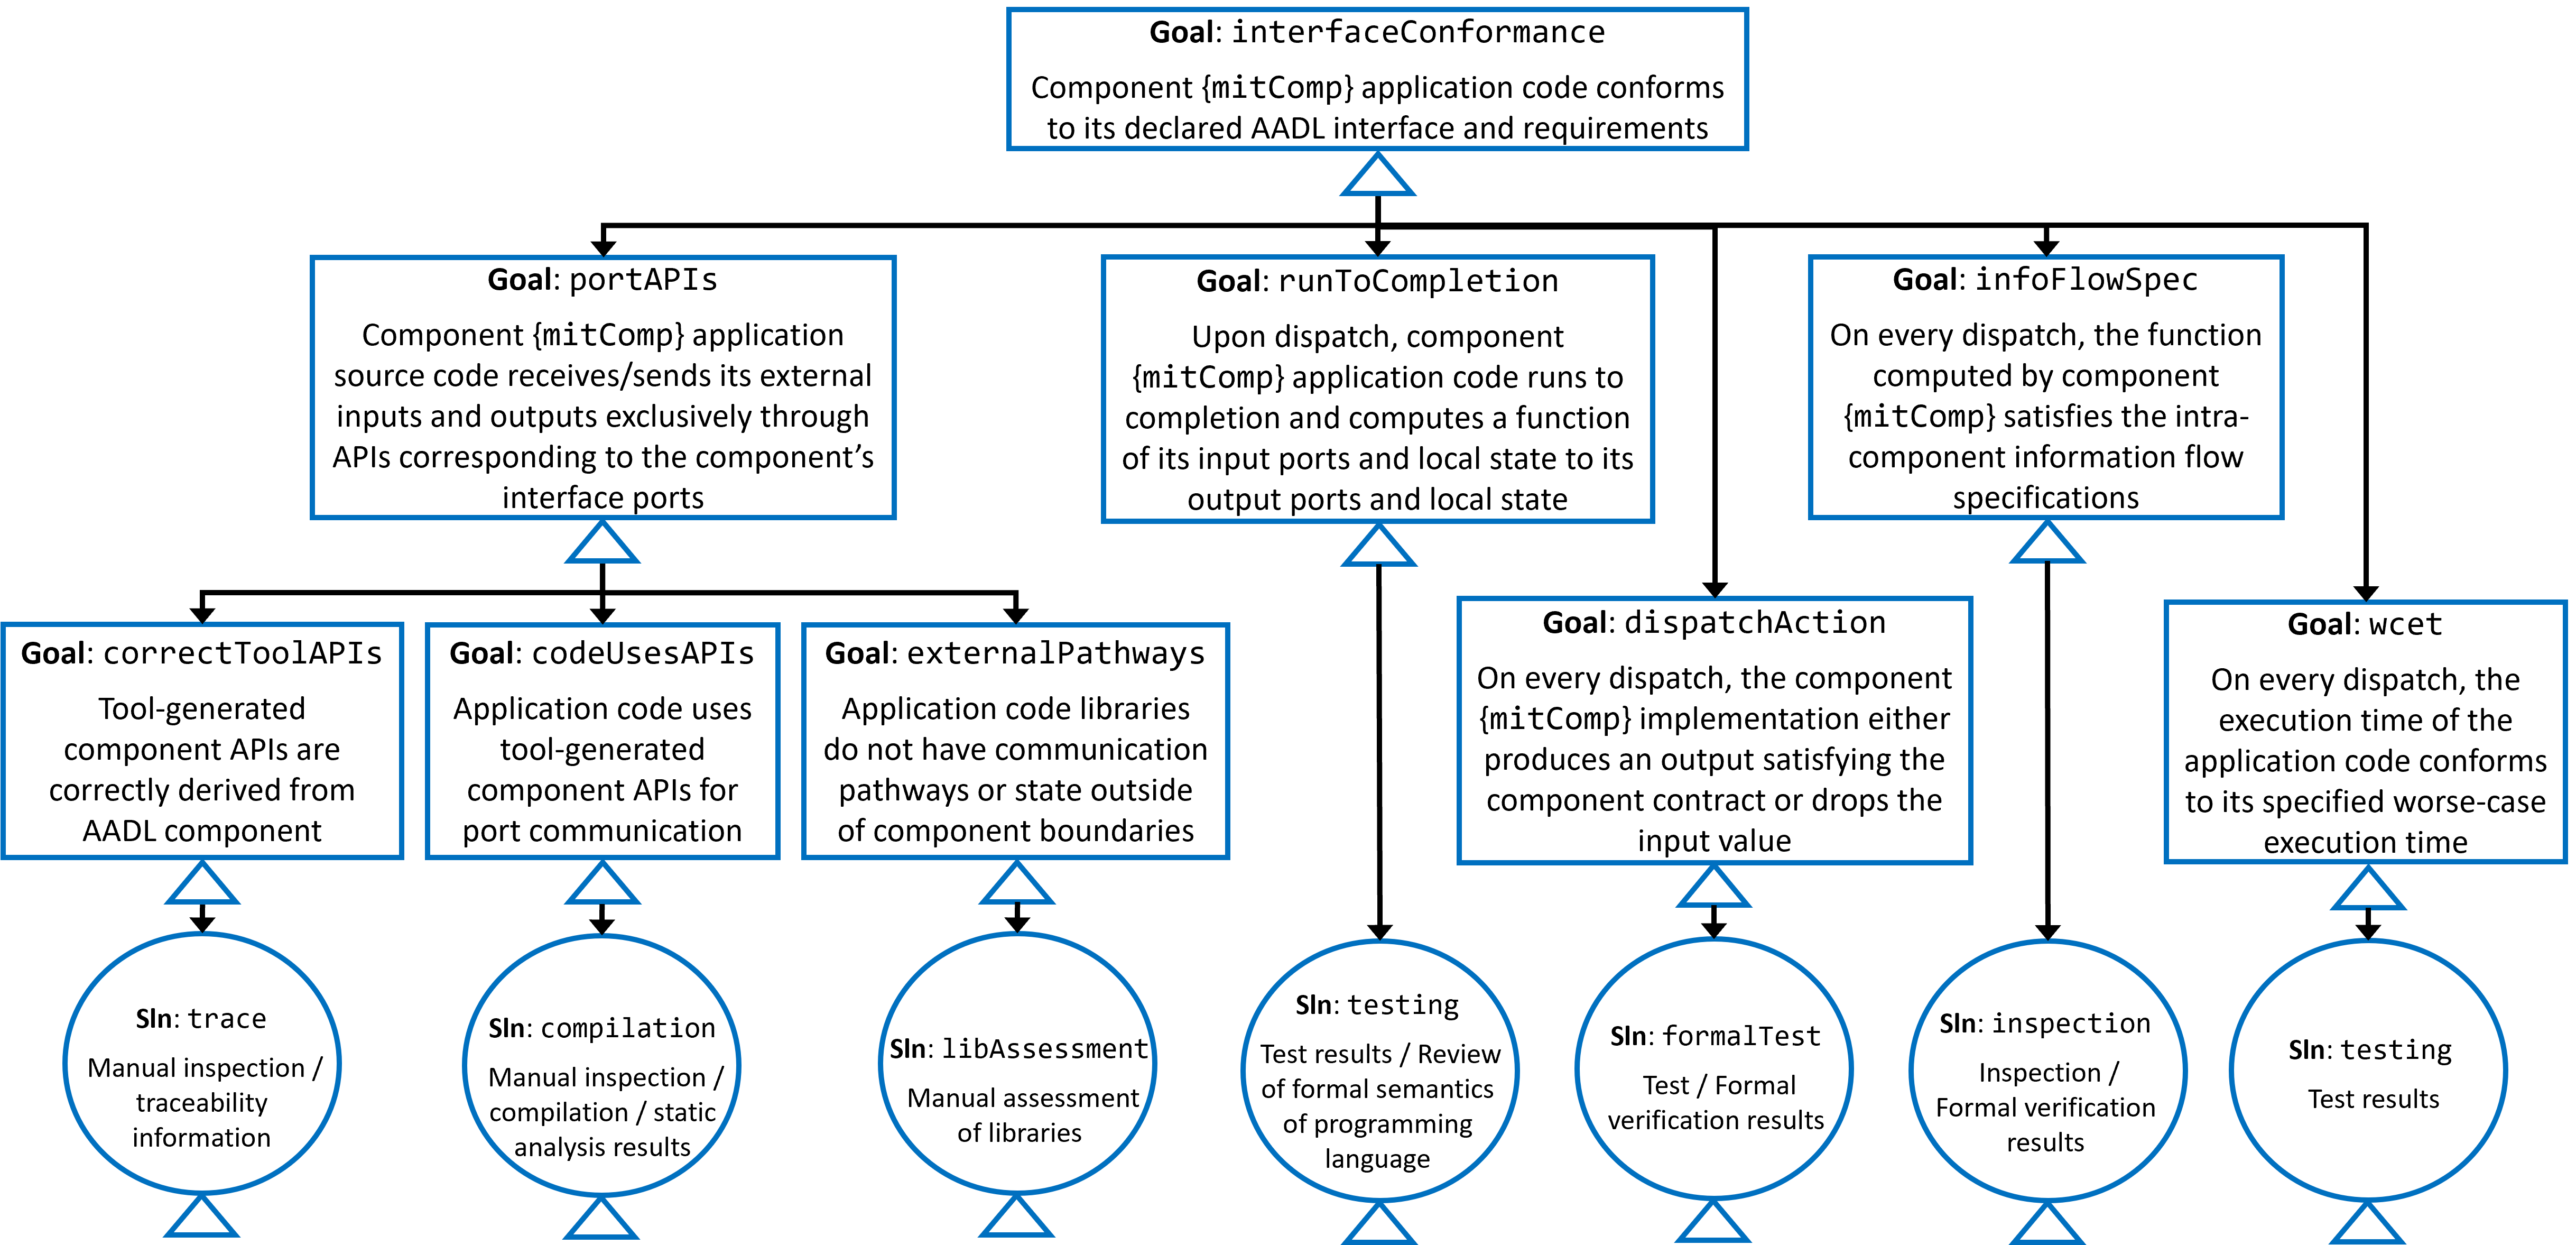
\includegraphics[width=\textwidth]{figs/code-conforms-to-interface-and-requirements.png}
	\caption{Assurance pattern for arguing component code conforms to the specified interface and requirements.}
	\label{fig:code-conforms-to-interface-and-requirements} 
\end{figure}

For goal \texttt{G???}, to demonstrate that the component's AADL runtime infrastructure code satisfies AADL port and threading semantics, we must show that for each component port declared in the AADL model, HAMR correctly generates (a) an API for application code (aligned with the AADL standard) to use when interacting with that port that is aligned with the AADL standard's description of port semantics, and (b) an implementation of the port API (aligned with the AADL standard's description of port semantics) that communicates values between the application code APIs and the boundary of the platform deployment of the component.  
%The port implementation achieves appropriate queuing and communication behavior in terms of the target platform's communication primitives.
Evidence to substantiate these claims comes from manual inspection of model-to-code traceability information as well as a justification of alignment with the AADL standard.

Finally, it must be shown that the component's platform deployment context achieves its required assurance properties (goal \texttt{G???}).  This is supported by the argument in Fig.~\ref{fig:platform-deployment-context-achieves-assurance-properties}.
\todo{Complete this argument description and required evidence}

\begin{figure}[h] 
	\centering 
	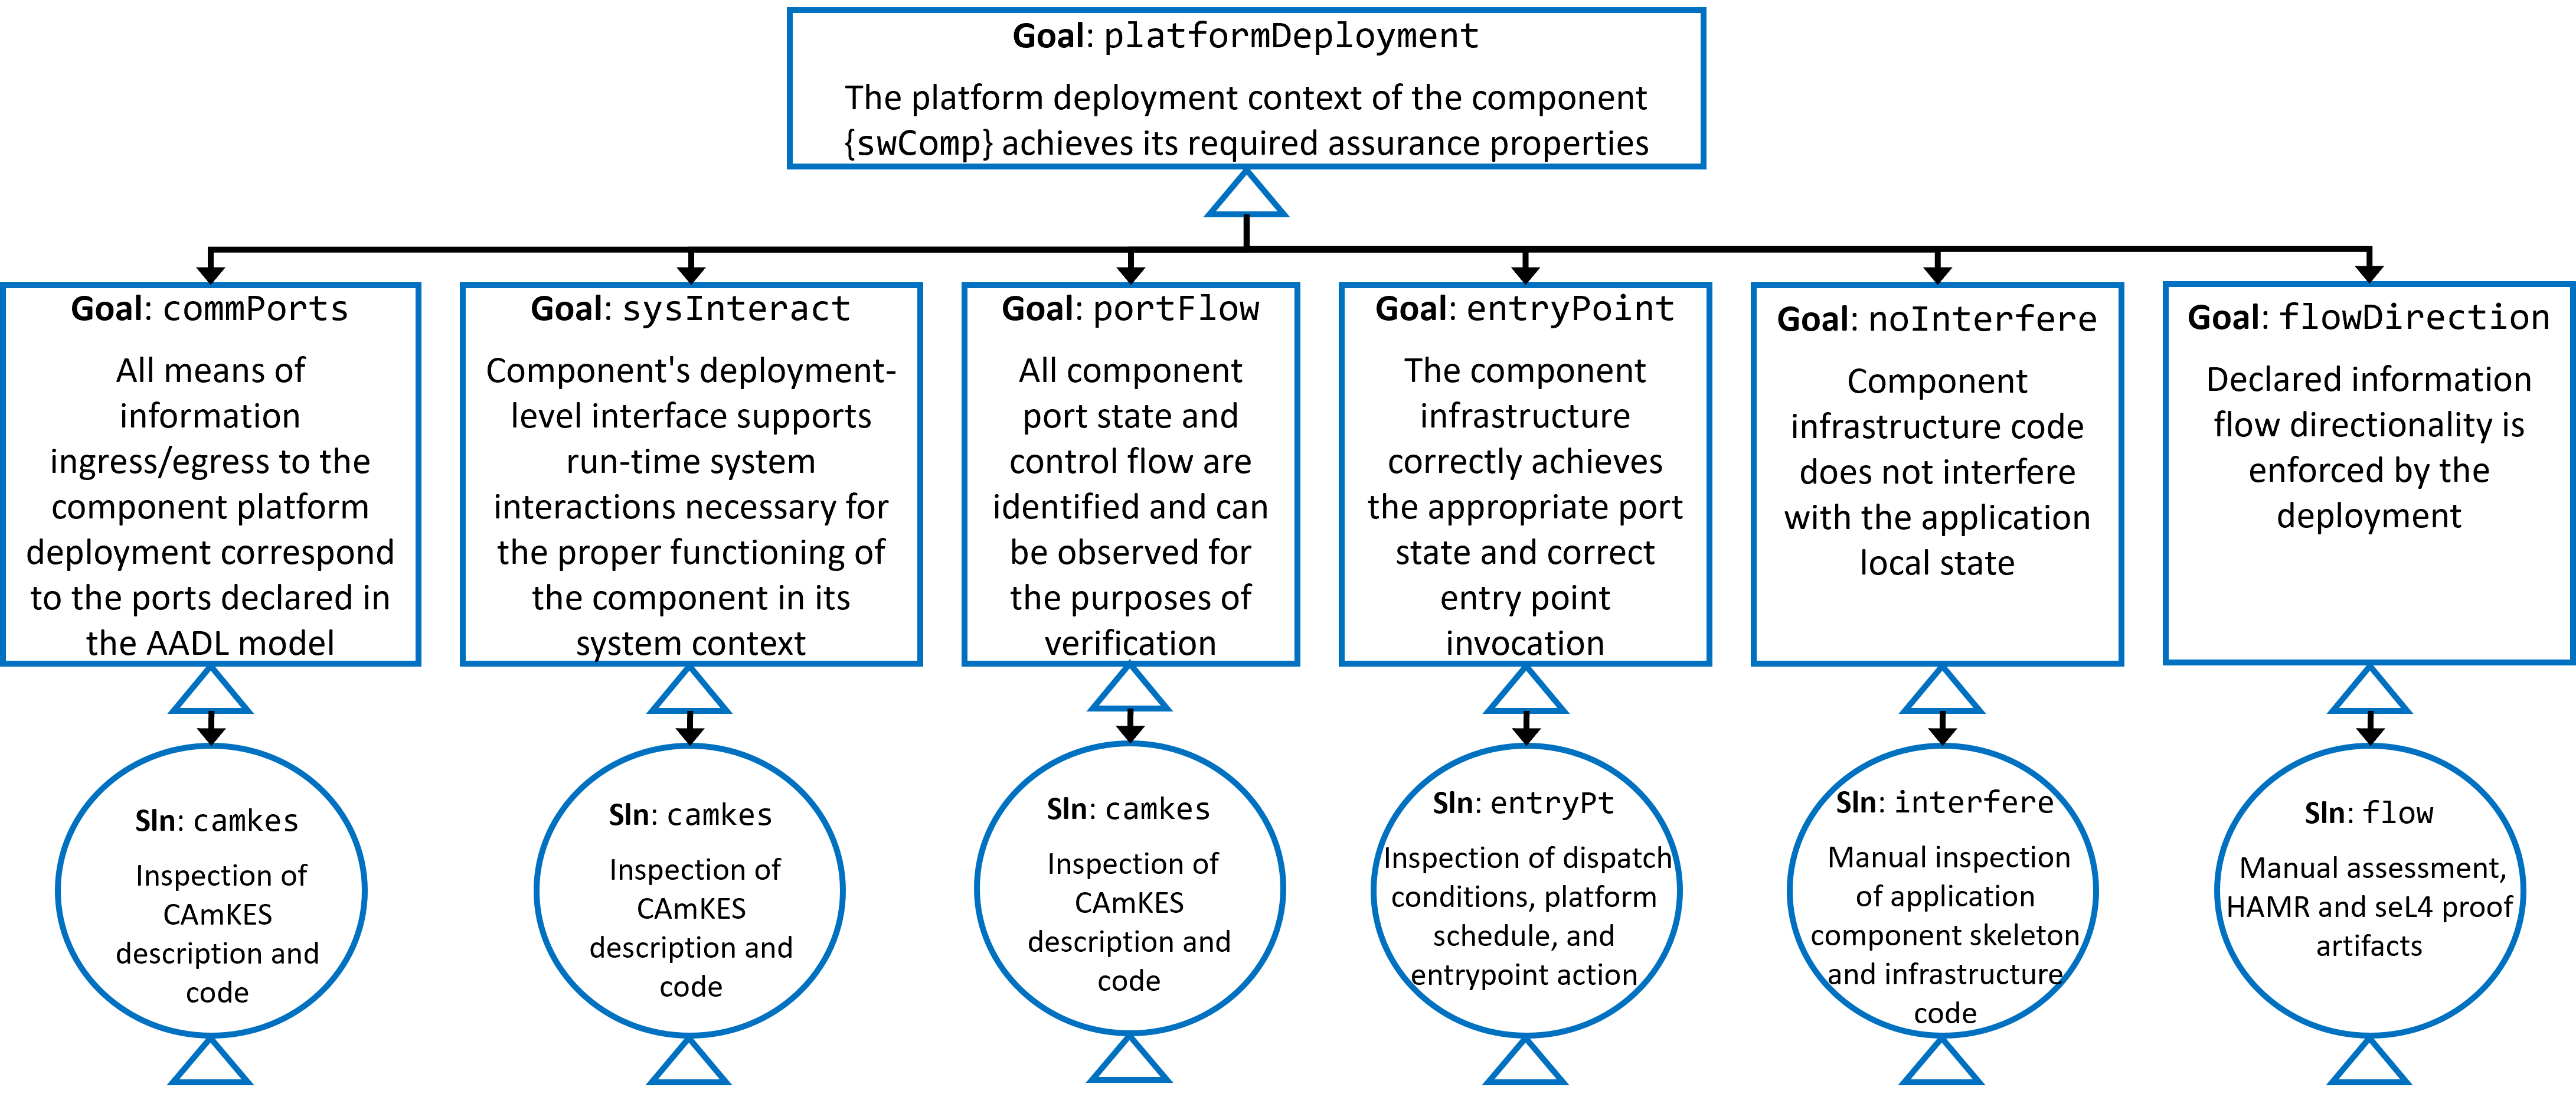
\includegraphics[width=\textwidth]{figs/platform-deployment-context-achieves-assurance-properties.png}
	\caption{Assurance pattern for arguing platform deployment context achieves the required assurance properties.}
	\label{fig:platform-deployment-context-achieves-assurance-properties} 
\end{figure}


In addition to demonstrating that \textit{deployed} software components satisfy their requirements, we must also argue that the platform components guarantee their required properties and the system implementation preserves them.
\todo{Complete this argument description and required evidence}